% \pagebreak[4]
% \hspace*{1cm}
% \pagebreak[4]
% \hspace*{1cm}
% \pagebreak[4]

\chapter{Theoretical background}
\ifpdf
    \graphicspath{{02_Theory/plots/}}
\else
    \graphicspath{{02_Theory/plots/EPS/}{02_Theory/plots/}}
\fi

\section{Standard Model}
Yet to be written...

% Here is an equation\footnote{the notation is explained in the nomenclature section :-)}:
% \begin{eqnarray}
% CIF: \hspace*{5mm}F_0^j(a) &=& \frac{1}{2\pi \iota} \oint_{\gamma} \frac{F_0^j(z)}{z - a} dz
% \end{eqnarray}
% \nomenclature[zcif]{$CIF$}{Cauchy's Integral Formula}                                % first letter Z is for Acronyms 
% \nomenclature[aF]{$F$}{complex function}                                                   % first letter A is for Roman symbols
% \nomenclature[gp]{$\pi$}{ $\simeq 3.14\ldots$}                                             % first letter G is for Greek Symbols
% \nomenclature[gi]{$\iota$}{unit imaginary number $\sqrt{-1}$}                      % first letter G is for Greek Symbols
% \nomenclature[gg]{$\gamma$}{a simply closed curve on a complex plane}  % first letter G is for Greek Symbols
% \nomenclature[xi]{$\oint_\gamma$}{integration around a curve $\gamma$} % first letter X is for Other Symbols
% \nomenclature[rj]{$j$}{superscript index}                                                       % first letter R is for superscripts
% \nomenclature[s0]{$0$}{subscript index}                                                        % first letter S is for subscripts

% \begin{figure}[!htbp]
%   \begin{center}
%     \leavevmode
%     \ifpdf
%       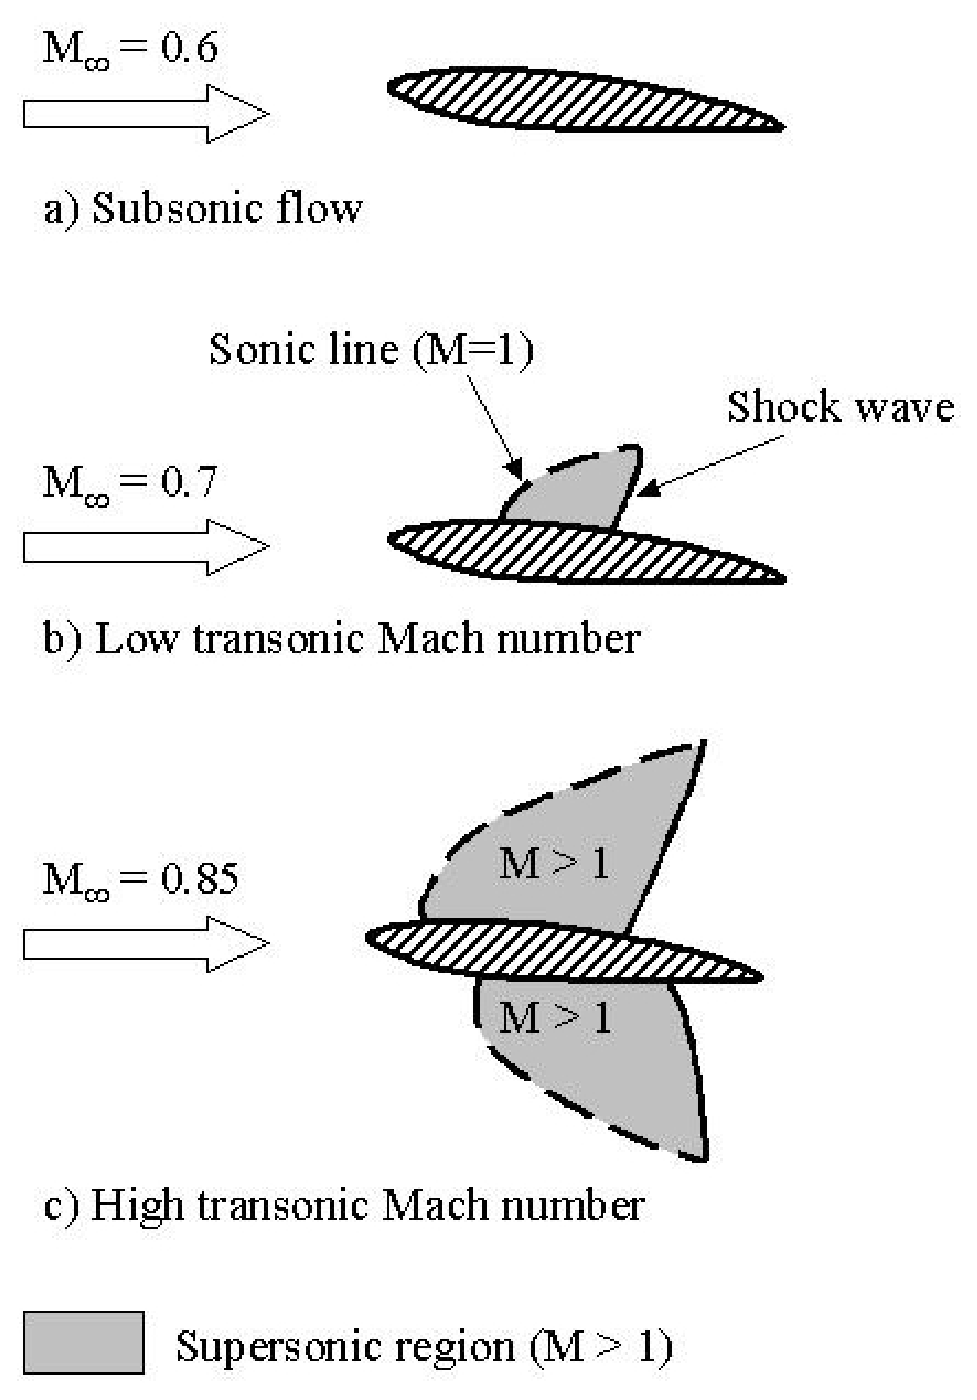
\includegraphics[height=6in]{aflow}
%     \else
%       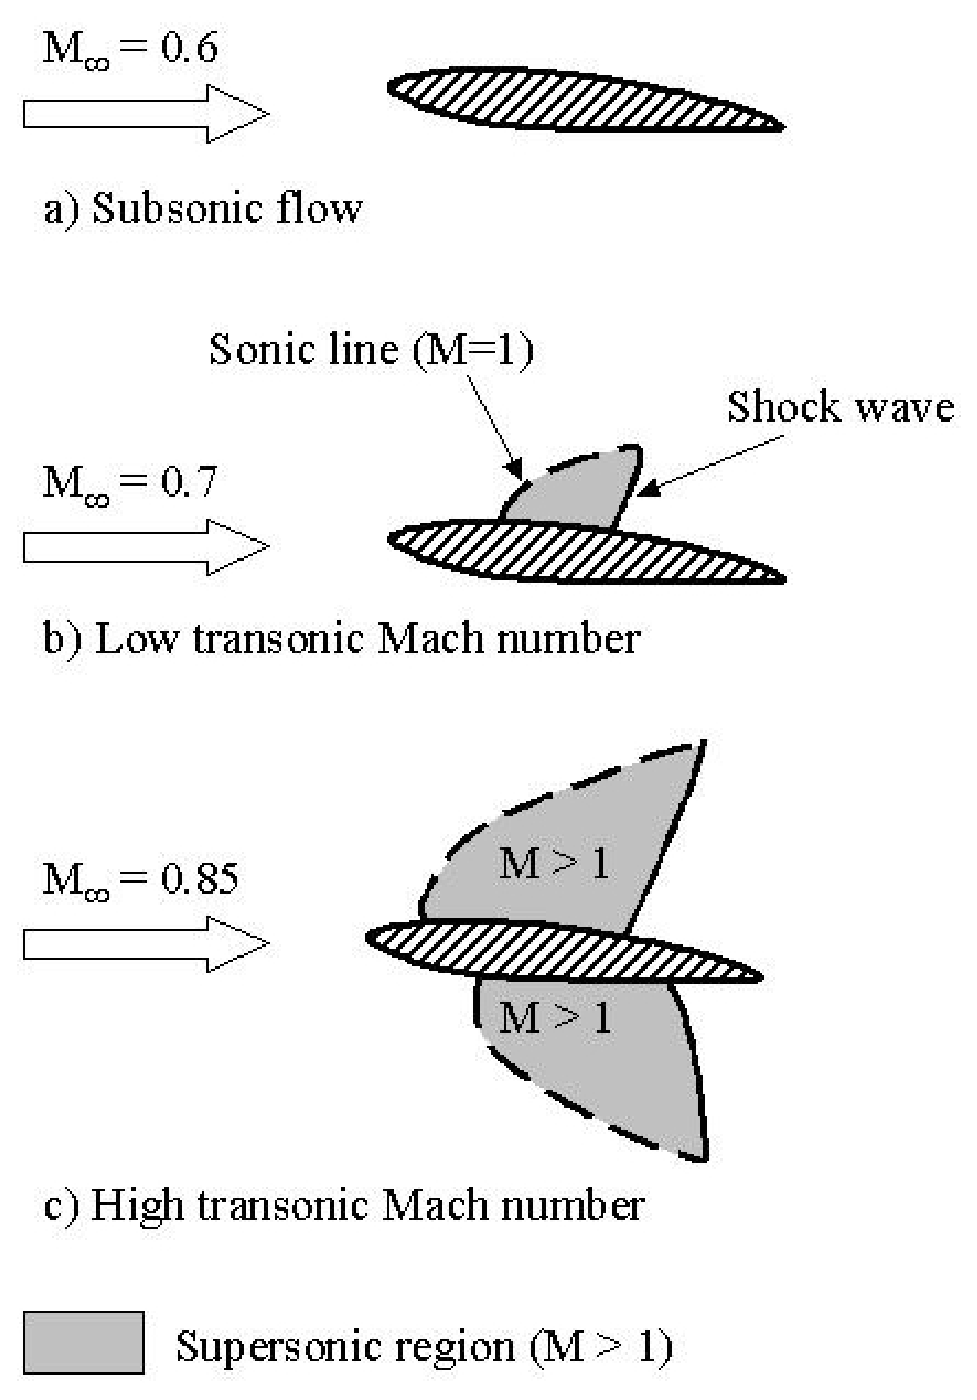
\includegraphics[bb = 92 86 545 742, height=6in]{aflow}
%     \fi
%     \caption{Airfoil Picture}
%     \label{FigAir}
%   \end{center}
% \end{figure}

%\InsertFig{\IncludeGraphicsH{aflow}{6in}{92 86 545 742}}{Airfoil Picture}{FigAir}
% So as we have now labelled it we can reference it, like so (\ref{FigAir}) and it
% is on Page \pageref{FigAir}. 
% ------------------------------------------------------------------------


%%% Local Variables: 
%%% mode: latex
%%% TeX-master: "../thesis"
%%% End: 
